\chapter{Background}
\label{sec:background}

Before going further in the implemented solutions, it's better to introduce a few background concepts. In particular, concepts about how FPGAs works, what kind of radiations exists and how FPGAs are affected by them.  

\section{Hardware Technology}

\subsection{FPGA Architecture}
\textit{FPGAs} (Field Programmable Gate Arrays) are used in a wide range of applications, from signal processing to machine learning applications. In particular, it is an integrated circuit designed to be general purpose: after manufacturing, it has no funcionalities. It is a hardware that can be programmed to perform specific tasks. \bigskip

It differs from a CPU. A CPU is an already designed hardware that is designed to do only one thing in a very optimized way: execute code, from a pre-defined Instruction Set. In this case, the action of \textit{programming} is referred to the process of writing a series of instructions that the CPU will eventually execute. This is done by exploiting Programming Languges. A FPGA, instead, is like LEGO bricks. Each LEGO brick alone does not have any function or purpose, but when assembled (so put together with other bricks), it can be used to perform a specific task. Here, the action of \textit{programming} is referred to the process of writing a \textit{description} on how all the bricks will be assembled to perform the specific task we want. The description is done exploiting Hardware Description Languages (HDL) like VHDL or Verilog. \bigskip

The basic FPGA design conists of I/O pads (to connect with the outside world), a set of routing channels and a set of LEGO bricks. A LEGO brick in the FPGA is a logic block (and depending on the vendor, it can be called CLB or LAB) that can be programmed to perform a very specific task that in the overall design helps in achieving the goal of the User's Application. 

\begin{figure}[H]
\centering
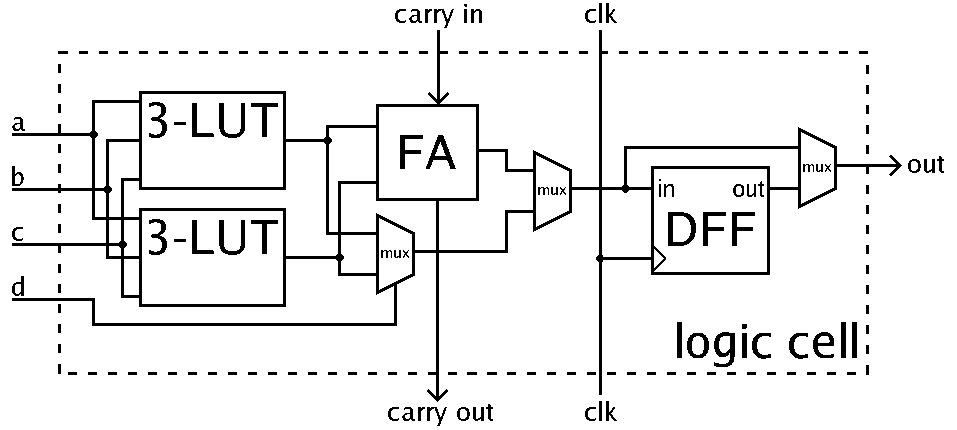
\includegraphics[width=1.0\linewidth]{images/chapter2/FPGA_cell_example.png}
\caption{Simplified schematic of a FPGA cell}
\label{fig:fpga_cell}
\end{figure}

A basic logic block consists of a few Logic Elements. As shown in figure \ref{fig:fpga_cell}, a Logic Elements is made of LUTs, a Full-Adder (FA), a D-Type Flip Flop and a bunch of multiplexers. This particular architecture can work in two modes: \textit{normal} mode and \textit{arithmetic} mode. Thanks to the Flip Flop, FPGAs can implement operations where some kind of memory is required.\bigskip

Modern FPGAs are very complex and expand upon the above capabilities to include other functionalities in silicon. Having these common functions embedded in the circuit reduces the area required and gives those functions increased speed compared to building them from logical primitives (because are implemented in-silicon, built out of transistor instead of LUTs, so they have ASICs-level performance). Examples of these include multipliers, generic DSP blocks, embedded processors, high speed I/O logic (like PCI/PCI-Express controllers, DRAM Controllers and so on and so forth) and embedded memories. \bigskip

Once the User's Application is designed (i.e. the description of the FPGA is written), the design needs to be mapped onto the FPGA's hardware resources. This is done using the Vendor's specific software and it's in charge of deciding which FPGA's LE is assigned to which subpart of the description and how each LE is configured. Then, all the LEs needs to be connected between themselfs and the I/O pads, and this is done by routing algorithms that decides the best way to connect them. Once all the implementation steps are done, a configuration file is generated that will eventually used to program the FPGA and is called \textit{bitstream}.\bigskip

All the programmable bits (like the content of the LUTs, some multiplexers selection signals or the routing details) are stored in the FPGA in memory elements that are outside the FPGA's funcional blocks (i.e. the one that can be used by the user to implement the application). Those memory elements can be though of as a big array of bits, or a \textit{shift register}. It's the \textit{configuration memory}: it stores the configuration bits of the entire FPGA and is loaded with the bitstream when the FPGA itself is programmed. Most FPGAs rely on an SRAM-based approach to be programmed: this allows to be in-system programmable (so the FPGA chip can be programmed without unmounting it from the board and from the system itself) and re-programmable (can be programmed as many times we want), but require external boot devices. Because the SRAM is a volatile memory, when the FPGA is powered off, the configuration memory content is lost. An external memory where the bitstream can be retrieved is required in order to re-program it. The SRAM approach is based on CMOS.\bigskip

Consequently, FPGAs are alternatives to hard-core CPUs. This means that on a FPGA a CPU can be implemented out of logic primitives (called \textit{soft-core}), alongside with the hardware that is used to implement the application like peripherals, memory and other components. Modern FPGAs supports \textit{at runtime programming}, this lead to the idea of \textit{reconfigurable systems}, where for example a CPU can be reconfigured in order to enable/disable some of its functionalities to suit the task at hand. The concept of \textit{reconfigurable systems} is also used in another manner and will be explained further in the next chapters.

\subsection{FPGAs vs. ASICs in Aerospace Applications}

An \textit{ASIC} (application-specific integrated circuit) is an integrated circuit chip customized for a particular use. ASIC chips are typically fabricated using metal-oxide-semiconductor (MOS) technology. Thanks to the miniaturization of the MOS-based transistors and the improvement in the design tools, the maximum complexity (and hence functionality) possible in an ASIC has grown from 5000 logic gates to over 100 million. \bigskip

This allows to implement entire microprocessors, memories (including ROM, RAM, EEPROM and flash) and other large component in a single chip. Usually, for lower production volumes, FPGAs may be more cost-effective than an ASIC design. This is due to the non-recurring engineering (NRE) cost of an ASIC, that can run into millions of dollars. \bigskip

1. what asics are
2. how they differs from fpgas
3. why fpga are better in aerospace applications (flexibility, needs to certificate only 1 piece of chip and the hardware can change during the development of the system, ability to reprogram from remote during operational phase) or the fact that software and hardware development can be done in parallel instead of sequentially so faster development and test and implementation time


\section{Radiations}